%%%%%%%%%%%%%%%%%%%%%%%%%%%%%%%%%%%%%%%%%%%%%%%%%%%%%%%%%%%%%%%%%%%%%%%%%%%
% Chapter: Peripherals and Interfaces
% Reference platform: Raspberry Pi Pico (RP2040), simulated in Wokwi.
% Examples: examples/interfaces/c (Arduino-Pico core + Pico SDK, runs in the
% browser) and examples/interfaces/rust (rp2040-hal, Wokwi for VS Code).
%%%%%%%%%%%%%%%%%%%%%%%%%%%%%%%%%%%%%%%%%%%%%%%%%%%%%%%%%%%%%%%%%%%%%%%%%%%

%%%%%%%%%%%%%%%%%%%%%%%%%%%%%%%%%%%%%%%%%%%%%%%%%%%%%%%%%%%%%%%%%%%%%%%%%%%
\section{Peripherals of a Microcontroller}
%%%%%%%%%%%%%%%%%%%%%%%%%%%%%%%%%%%%%%%%%%%%%%%%%%%%%%%%%%%%%%%%%%%%%%%%%%%
\nsl{A microcontroller is more than a processor core. Most of the chip area
is used by peripherals: blocks of hardware that talk to the outside world
on their own, such as GPIO ports, timers, PWM generators, analog-to-digital
converters and serial interfaces. The processor only configures them and
exchanges data with them. It does so by reading and writing registers that
appear at fixed addresses in the memory map.
\newline
In this chapter we use the Raspberry Pi Pico with the RP2040 microcontroller
as our reference platform. It is cheap, very well documented and, most
importantly for the lecture, it can be simulated completely in the browser
with Wokwi. All examples exist in two versions: in C using the Pico SDK
(running in the browser) and in Rust using the rp2040-hal crate (built
locally and simulated in Wokwi for VS Code). The concepts carry over to any
other microcontroller; only register names and addresses change.
\newpage}

\begin{description}
\item[{\rot\bf The reference platform: RP2040 / Raspberry Pi Pico}]~\\[-3ex]
\bi
	\ite two ARM Cortex-M0+ cores, 125\,MHz (up to 200\,MHz), 264\,KB SRAM, program in external QSPI flash (2\,MB on the Pico)
	\ite 30 GPIO pins (26 usable on the Pico), 3.3\,V logic, \textbf{not} 5\,V tolerant
	\ite peripherals
	\bi
		\ite 2 $\times$ UART, 2 $\times$ I$^2$C, 2 $\times$ SPI, USB 1.1 (device and host)
		\ite 8 PWM slices with 2 outputs each (16 PWM channels)
		\ite 12 bit ADC with 4 external inputs and an internal temperature sensor
		\ite 64 bit microsecond timer with 4 alarms, watchdog, real-time clock
		\ite 12 DMA channels, 2 PIO blocks (programmable I/O state machines)
	\ei
\ei
\os{\newpage}

\item[{\rot\bf Memory-mapped I/O}]~\\[-3ex]
\bi
	\ite every peripheral is a block of \textbf{registers} in the address space
	\ite the CPU accesses them with normal load/store instructions
	\ite typical kinds of registers
	\bi
		\ite \textbf{control} registers: mode, enable, speed, \ldots
		\ite \textbf{status} registers: flags like ``data received'', ``FIFO full''
		\ite \textbf{data} registers: the values transferred to or from the outside world
	\ei
	\ite a register is not memory: reading may clear a flag, writing may start an action
	\bi
		\ite in C every access has to be \texttt{volatile}, otherwise the compiler may remove or merge it
	\ei
\ei

\begin{figure}[!hbtp]
\begin{center}
\resizebox{0.8\textwidth}{!}{%
\begin{tikzpicture}[font=\sffamily\small,
	box/.style={draw,thick,minimum height=9mm,minimum width=22mm,align=center},
	>=Stealth]
	\node[box,fill=blue!10] (cpu) at (0,0) {CPU\\Cortex-M0+};
	\node[box,fill=gray!10,minimum width=24mm] (mem) at (0,-2.2) {Flash / SRAM};
	\draw[very thick] (2,1.2) -- (2,-3.2) node[below]{bus};
	\draw[<->,thick] (cpu) -- (2,0);
	\draw[<->,thick] (mem) -- (2,-2.2);
	\foreach \name/\y/\addr in {GPIO/1/0x4001\,4000, UART0/0/0x4003\,4000, I2C0/-1/0x4004\,4000, ADC/-2/0x4004\,c000, PWM/-3/0x4005\,0000}{
		\node[box,fill=orange!15,anchor=west] (p\name) at (3,\y) {\name};
		\draw[<->,thick] (2,\y) -- (p\name);
		\node[anchor=west,font=\sffamily\scriptsize] at ($(p\name.east)+(0.1,0)$) {\addr};
	}
	\node[anchor=west,font=\sffamily\scriptsize] at (5.4,1.6) {base address};
\end{tikzpicture}}
\caption{Peripherals are register blocks in the memory map (RP2040 addresses)}
\end{center}
\end{figure}
\os{\newpage}

\item[{\rot\bf Before a peripheral can be used}]~\\[-3ex]
\bi
	\ite release it from \textbf{reset} (most blocks start in reset to save power)
	\ite make sure it gets a \textbf{clock} (e.g.\ \texttt{clk\_peri} for UART and SPI)
	\ite connect it to the pins: \textbf{pin multiplexing}
	\bi
		\ite a pin has many possible functions, but only one at a time
		\ite on the RP2040: \texttt{FUNCSEL} field in the register \texttt{GPIOn\_CTRL}
		\ite e.g.\ GP0 can be SPI0 RX, UART0 TX, I2C0 SDA, PWM0 A, SIO (software GPIO), PIO, \ldots
	\ei
	\ite configure the peripheral, then enable it
	\ite the SDK (C) and the HAL (Rust) do these steps for us -- but they still happen
\ei
\os{\newpage}

\item[{\rot\bf Polling, interrupts and DMA}]~\\[-3ex]
\bi
	\ite \textbf{polling}: the program checks a status flag in a loop
	\bi
		\ite simple and predictable, but the CPU is busy while waiting
	\ei
	\ite \textbf{interrupt}: the peripheral signals an event, the CPU interrupts the running program and executes an interrupt service routine (ISR)
	\bi
		\ite the CPU can sleep or do other work in between
		\ite shared data between ISR and main program needs care
	\ei
	\ite \textbf{DMA} (direct memory access): a separate controller copies data between peripheral and memory
	\bi
		\ite the CPU only sets up the transfer and is informed at the end
		\ite used for fast or continuous data streams (ADC sampling, displays, audio)
	\ei
\ei
\os{\newpage}

\item[{\rot\bf Our simulated circuit (Wokwi)}]~\\[-3ex]
\bi
	\ite one circuit for all examples of this chapter: \texttt{examples/interfaces/diagram.json}
\ei
\begin{center}
\resizebox{\textwidth}{!}{%
\begin{tabular}{|l|l|l|}
\hline
\textbf{Pico pin} & \textbf{connected to} & \textbf{peripheral} \\
\hline
GP0 / GP1 & serial monitor & UART0 TX / RX \\
GP4 / GP5 & MPU6050 acceleration sensor & I2C0 SDA / SCL \\
GP14 & push button to GND & GPIO input \\
GP15 & LED with 220\,$\Omega$ resistor & GPIO output, PWM7 B \\
GP17 / GP18 / GP19 & 74HC595 shift register + LED bar & GPIO latch, SPI0 SCK / TX \\
GP26 & potentiometer & ADC0 \\
\hline
\end{tabular}}
\end{center}
\bi
	\ite a logic analyzer records 8 of these signals (export as VCD file)
	\ite C: paste sketch and \texttt{diagram.json} into a new Pico project on \url{https://wokwi.com}
	\ite Rust: \texttt{cargo build --release}, then start the simulation with the Wokwi extension in VS Code
\ei
\os{\newpage}
\end{description}

%%%%%%%%%%%%%%%%%%%%%%%%%%%%%%%%%%%%%%%%%%%%%%%%%%%%%%%%%%%%%%%%%%%%%%%%%%%
\section{Digital Inputs and Outputs (GPIO)}
%%%%%%%%%%%%%%%%%%%%%%%%%%%%%%%%%%%%%%%%%%%%%%%%%%%%%%%%%%%%%%%%%%%%%%%%%%%
\nsl{General purpose input/output (GPIO) is the simplest interface: the
software decides whether a pin drives a level (output) or reads one (input).
Even this simple case shows the typical structure of every peripheral. There
is a multiplexer that connects the pin to one of several internal functions,
a pad with electrical options such as pull resistors and drive strength,
and registers to control everything.}

\begin{description}
\item[{\rot\bf Structure of a GPIO pin}]~\\[-3ex]
\begin{figure}[!hbtp]
\begin{center}
\resizebox{0.9\textwidth}{!}{%
\begin{tikzpicture}[font=\sffamily\small,
	box/.style={draw,thick,minimum height=8mm,align=center},
	>=Stealth]
	\node[box,minimum width=20mm,fill=blue!10] (sio) at (0,1.5) {SIO\\(software)};
	\node[box,minimum width=20mm,fill=orange!15] (uart) at (0,0) {UART, SPI,\\I2C, PWM};
	\node[box,minimum width=20mm,fill=gray!10] (pio) at (0,-1.5) {PIO, USB, \ldots};
	\node[box,minimum width=16mm,minimum height=42mm,fill=yellow!20] (mux) at (3.5,0) {FUNCSEL\\multiplexer\\(IO\_BANK0)};
	\foreach \n in {sio,uart,pio} \draw[<->,thick] (\n.east) -- (\n.east -| mux.west);
	\node[box,minimum width=26mm,minimum height=42mm,fill=green!10,align=left] (pad) at (7.2,0)
		{\textbf{Pad} (PADS\_BANK0)\\[1mm] output enable\\drive strength 2..12\,mA\\slew rate\\pull-up / pull-down\\Schmitt trigger\\input enable};
	\draw[<->,thick] (mux) -- (pad);
	\draw[very thick] (pad.east) -- ++(1.2,0) node[draw,circle,fill=white,inner sep=2pt,label=above:{pin GPn}] {};
\end{tikzpicture}}
\caption{Path from the peripherals to a GPIO pin of the RP2040}
\end{center}
\end{figure}
\bi
	\ite FUNCSEL = 5 connects the pin to the \textbf{SIO} (single-cycle I/O): the CPU controls it directly
	\ite the pad settings are independent of the selected function
\ei
\os{\newpage}

\item[{\rot\bf SIO registers for GPIO (base address 0xd000\,0000)}]~\\[-3ex]
\begin{center}
\resizebox{\textwidth}{!}{%
\begin{tabular}{|l|l|l|}
\hline
\textbf{Offset} & \textbf{Register} & \textbf{Meaning (one bit per pin)} \\
\hline
0x004 & GPIO\_IN & input levels \\
0x010 & GPIO\_OUT & output values \\
0x014, 0x018, 0x01c & GPIO\_OUT\_SET, \_CLR, \_XOR & set / clear / toggle output bits \\
0x020 & GPIO\_OE & output enable (1 = output) \\
0x024, 0x028, 0x02c & GPIO\_OE\_SET, \_CLR, \_XOR & set / clear / toggle enable bits \\
\hline
\end{tabular}}
\end{center}
\bi
	\ite why SET, CLR and XOR registers?
	\bi
		\ite \texttt{GPIO\_OUT |= (1 << 15)} is a read-modify-write: three instructions
		\ite if an interrupt (or the second core) changes another bit in between, that change is lost
		\ite writing \texttt{1 << 15} to GPIO\_OUT\_SET changes only bit 15, in one bus access
	\ei
	\ite the other peripherals of the RP2040 offer the same idea for every register: aliases at +0x1000 (XOR), +0x2000 (SET), +0x3000 (CLR)
\ei
\os{\newpage}

\item[{\rot\bf Blinking with raw register accesses (C)}]~\\[-3ex]
\begin{lstlisting}[language=C]
#define IO_BANK0_ADDR   0x40014000u
#define SIO_ADDR        0xd0000000u

// GPIOn_CTRL: function select of pin n (8 bytes per pin, CTRL at offset 4)
#define GPIO_CTRL(n)    (*(volatile uint32_t *)(IO_BANK0_ADDR + 0x04u + 8u * (n)))
#define SIO_GPIO_OE_SET (*(volatile uint32_t *)(SIO_ADDR + 0x024u))
#define SIO_GPIO_OUT_XOR (*(volatile uint32_t *)(SIO_ADDR + 0x01cu))

#define FUNCSEL_SIO     5u
#define LED             15u

void setup() {
  GPIO_CTRL(LED)  = FUNCSEL_SIO;   // pin is controlled by software (SIO)
  SIO_GPIO_OE_SET = 1u << LED;     // enable output driver (atomic set)
}

void loop() {
  SIO_GPIO_OUT_XOR = 1u << LED;    // toggle - no read-modify-write needed
  delay(500);
}
\end{lstlisting}
\os{\newpage}

\item[{\rot\bf The same with the Pico SDK (C)}]~\\[-3ex]
\begin{lstlisting}[language=C]
#include "hardware/gpio.h"

const uint LED = 15;

void setup() {
  gpio_init(LED);               // FUNCSEL = SIO, output disabled, value 0
  gpio_set_dir(LED, GPIO_OUT);  // enable the output driver
}

void loop() {
  gpio_put(LED, 1);
  sleep_ms(500);
  gpio_put(LED, 0);
  sleep_ms(500);
}
\end{lstlisting}
\bi
	\ite the SDK functions are thin wrappers around the registers shown before
	\ite \texttt{gpio\_put()} writes to GPIO\_OUT\_SET or GPIO\_OUT\_CLR
\ei
\os{\newpage}

\item[{\rot\bf The same in Rust (rp2040-hal)}]~\\[-3ex]
\begin{lstlisting}[language=Rust]
#[entry]
fn main() -> ! {
    // Take ownership of the peripherals - exactly once.
    let mut pac = pac::Peripherals::take().unwrap();
    // ... clock setup (12 MHz crystal -> PLL -> 125 MHz) ...
    let sio = hal::Sio::new(pac.SIO);
    let pins = rp_pico::Pins::new(pac.IO_BANK0, pac.PADS_BANK0, sio.gpio_bank0, &mut pac.RESETS);

    // The type system knows that this pin is now a push-pull output.
    let mut led = pins.gpio15.into_push_pull_output();

    loop {
        led.set_high().unwrap();
        delay.delay_ms(500);
        led.set_low().unwrap();
        delay.delay_ms(500);
    }
}
\end{lstlisting}
\os{\newpage}

\item[{\rot\bf What Rust adds: ownership and type states}]~\\[-3ex]
\bi
	\ite \texttt{Peripherals::take()} returns the peripherals only on the first call
	\bi
		\ite there is exactly one owner of each register block, so two parts of the program cannot configure the same peripheral by accident
	\ei
	\ite the configuration of a pin is part of its \textbf{type}
	\bi
		\ite \texttt{pins.gpio15} has the type \texttt{Pin<Gpio15, FunctionNull, PullDown>}
		\ite \texttt{into\_push\_pull\_output()} consumes it and returns \texttt{Pin<Gpio15, FunctionSioOutput, PullDown>}
		\ite \texttt{set\_high()} only exists for output pins: writing to an input pin is a \textbf{compile error}, not a bug found on the hardware
		\ite after \texttt{into\_function::<FunctionUart>()} the pin can only be handed to a UART
	\ei
	\ite all of this is checked by the compiler and costs nothing at run time
	\ite raw register access is still possible, but must be marked \texttt{unsafe} (see \texttt{gpio\_blink\_registers.rs})
\ei
\os{\newpage}

\item[{\rot\bf Output stages}]~\\[-3ex]
\bi
	\ite \textbf{push-pull}: one transistor connects the pin to the supply, the other to GND
	\bi
		\ite drives both levels actively, fast edges in both directions
		\ite never connect two push-pull outputs: if one drives high and the other low, a large current flows and can destroy the pins
	\ei
\ei
\begin{figure}[!hbtp]
     \begin{center}
	  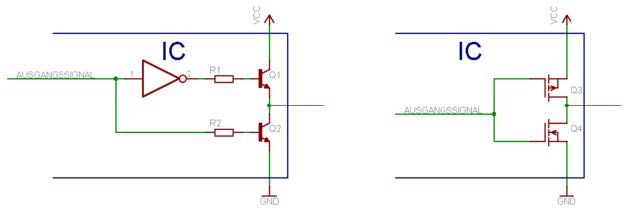
\epsfig{file=figures/PushPull.jpg,width=0.55\textwidth}\\
	  \caption{Push-pull output}
     \end{center}
\end{figure}
\os{\newpage}

\bi
	\ite \textbf{open drain} (open collector for bipolar transistors): only the transistor to GND exists
	\bi
		\ite the pin can only pull the line low; a resistor pulls it high
		\ite several outputs may share one line: it is low if any output pulls it low (``wired AND'')
		\ite the rising edge is slow, as the pull-up resistor charges the line capacitance ($\tau = RC$)
		\ite the high level may differ from the chip's supply (level shifting, e.g.\ 3.3\,V to 5\,V)
		\ite used for I$^2$C, interrupt lines, reset lines
	\ei
\ei
\begin{figure}[!hbtp]
     \begin{center}
	  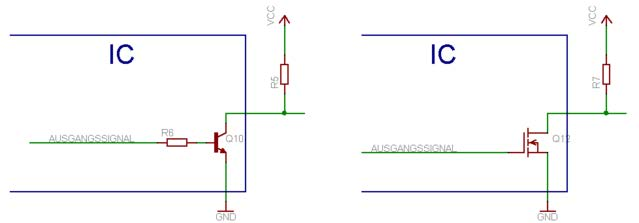
\epsfig{file=figures/OpenCollector.jpg,width=0.55\textwidth}\\
	  \caption{Open-drain output with external pull-up resistor}
     \end{center}
\end{figure}
\os{\newpage}

\bi
	\ite \textbf{tri-state}: a push-pull stage with an additional ``off'' state (high impedance, Z)
	\bi
		\ite in state Z the pin neither drives high nor low and behaves as if it were not connected
		\ite many devices can share a bus as long as only one of them drives at a time
		\ite on the RP2040: output enable = 0 means Z
		\ite open drain can be emulated: output value fixed at 0, switch only the output enable
	\ei
\ei
\begin{figure}[!hbtp]
     \begin{center}
	  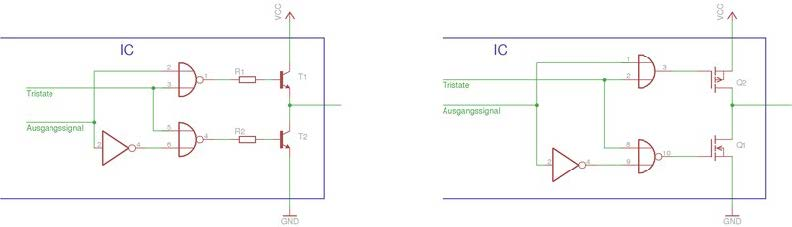
\epsfig{file=figures/TriState.jpg,width=0.55\textwidth}\\
	  \caption{Tri-state output}
     \end{center}
\end{figure}
\os{\newpage}

\item[{\rot\bf Inputs}]~\\[-3ex]
\bi
	\ite an unconnected (``floating'') input reads random values: it picks up noise
	\bi
		\ite always define the idle level with a pull-up or pull-down resistor
		\ite RP2040: internal pull-up / pull-down of about 50--80\,k$\Omega$ in the pad
	\ei
	\ite a typical button connects the pin to GND and uses the pull-up: \textbf{pressed = low}
	\ite \textbf{Schmitt trigger}: two switching thresholds (hysteresis), so a slowly changing or noisy signal gives one clean edge instead of many
	\ite electrical limits matter
	\bi
		\ite 3.3\,V maximum on any pin of the RP2040 -- a 5\,V signal needs a level shifter or voltage divider
		\ite drive strength 2, 4 (default), 8 or 12\,mA per pin -- enough for an LED, never for a motor or relay
	\ei
\ei
\os{\newpage}

\item[{\rot\bf Contact bounce}]~\\[-3ex]
\bi
	\ite mechanical contacts do not close cleanly: they bounce for some 100\,$\mu$s up to about 20\,ms
	\ite the software sees many edges for one press -- Wokwi simulates this as well
\ei
\begin{figure}[!hbtp]
\begin{center}
\resizebox{0.75\textwidth}{!}{%
\begin{tikztimingtable}[timing/slope=0.05, xscale=0.9, yscale=1.2, font=\sffamily\small]
	button (raw) & 4H 0.4L 0.3H 0.3L 0.2H 0.5L 0.15H 8L 0.2H 0.2L 0.3H 4H \\
	debounced    & 7.85H 8.7L 2H \\
\extracode
	\draw[decorate,decoration={brace,amplitude=4pt}] (4,0.4) -- node[above=4pt,font=\sffamily\scriptsize] {bounces} (5.85,0.4);
	\draw[<->] (5.85,-2.9) -- node[below,font=\sffamily\scriptsize] {stable for 20 ms} (7.85,-2.9);
\end{tikztimingtable}}
\caption{Bouncing button and debounced signal}
\end{center}
\end{figure}
\bi
	\ite hardware solution: RC low-pass filter followed by a Schmitt trigger
	\ite software solution: accept a new level only if it was stable for a certain time
\ei
\os{\newpage}

\item[{\rot\bf Debouncing in software (Rust)}]~\\[-3ex]
\begin{lstlisting}[language=Rust]
let mut led = pins.gpio15.into_push_pull_output();
// Button connects the pin to GND -> use the internal pull-up, pressed = low.
let mut button = pins.gpio14.into_pull_up_input();

let mut stable_pressed = false; // debounced state
let mut counter = 0; // how long the raw level differs from the stable state

loop {
    let raw_pressed = button.is_low().unwrap();
    if raw_pressed != stable_pressed {
        counter += 1;
        if counter >= STABLE_MS {
            stable_pressed = raw_pressed;
            counter = 0;
            if stable_pressed {
                led.toggle().unwrap(); // react on the press edge only
            }
        }
    } else {
        counter = 0;
    }
    delay.delay_ms(1); // sample every 1 ms
}
\end{lstlisting}
\bi
	\ite C version: \texttt{examples/interfaces/c/button\_debounce}
\ei
\os{\newpage}
\end{description}

%%%%%%%%%%%%%%%%%%%%%%%%%%%%%%%%%%%%%%%%%%%%%%%%%%%%%%%%%%%%%%%%%%%%%%%%%%%
\section{Interrupts}
%%%%%%%%%%%%%%%%%%%%%%%%%%%%%%%%%%%%%%%%%%%%%%%%%%%%%%%%%%%%%%%%%%%%%%%%%%%
\nsl{Polling a button every millisecond works, but it keeps the processor
busy and the reaction time depends on the loop. With an interrupt the
hardware itself watches the pin. When the selected edge occurs, the
processor finishes the current instruction, saves its state and jumps to
an interrupt service routine (ISR). Afterwards the interrupted program
continues as if nothing had happened. This is efficient, but it brings a
new class of errors. The ISR and the main program run ``at the same time''
from the program's point of view, so every variable they share must be
protected.}

\begin{description}
\item[{\rot\bf How an interrupt is handled on a Cortex-M}]~\\[-3ex]
\bi
	\ite the peripheral sets an interrupt flag (e.g.\ ``falling edge on GP14'')
	\ite if enabled, the request goes to the \textbf{NVIC} (nested vectored interrupt controller)
	\bi
		\ite RP2040: 32 interrupt lines per core, 4 priority levels
		\ite a higher priority interrupt can interrupt a running ISR (nesting)
	\ei
	\ite the core pushes registers onto the stack and loads the ISR address from the \textbf{vector table}
	\bi
		\ite latency on the Cortex-M0+: 15 clock cycles (120\,ns at 125\,MHz)
	\ei
	\ite the ISR must \textbf{clear the flag}, otherwise it is entered again immediately
	\ite on return the saved registers are restored automatically
\ei
\os{\newpage}

\item[{\rot\bf Rules for interrupt service routines}]~\\[-3ex]
\bi
	\ite keep ISRs \textbf{short}: set a flag, store a value, wake up a task
	\ite no blocking calls (delays, waiting for a UART, \texttt{printf}) inside an ISR
	\ite variables shared with the main program
	\bi
		\ite C: declare them \texttt{volatile}, so the compiler reads them from memory every time
		\ite \texttt{volatile} does \textbf{not} make an access atomic: a 64 bit value or a read-modify-write (\texttt{count++}) can still be interrupted in the middle
		\ite protect such accesses with a critical section (interrupts disabled for a short time)
	\ei
	\ite Rust enforces this: a \texttt{static} shared with an ISR must be wrapped, e.g.\ in a \texttt{Mutex} that can only be opened inside a critical section
\ei
\os{\newpage}

\item[{\rot\bf GPIO interrupt (C, Arduino API)}]~\\[-3ex]
\bi
	\ite try it: one press often gives several interrupts -- the bouncing is visible again
\ei
\begin{lstlisting}[language=C]
const int LED = 15, BUTTON = 14;
volatile uint32_t irqCount = 0;   // shared with the ISR -> volatile

void onButton() {                 // interrupt service routine: keep it short
  digitalWrite(LED, !digitalRead(LED));
  irqCount++;
}

void setup() {
  Serial1.begin(115200);
  pinMode(LED, OUTPUT);
  pinMode(BUTTON, INPUT_PULLUP);
  attachInterrupt(digitalPinToInterrupt(BUTTON), onButton, FALLING);
}
void loop() {
  static uint32_t last = 0;
  uint32_t now = irqCount;        // 32 bit read is atomic on the Cortex-M0+
  if (now != last) {
    Serial1.printf("interrupts so far: %lu\n", (unsigned long)now);
    last = now;
  }
}
\end{lstlisting}
\os{\newpage}

\item[{\rot\bf GPIO interrupt (Rust)}]~\\[-3ex]
\begin{lstlisting}[language=Rust]
// Hand-over main() -> ISR; the Mutex opens only in a critical section
static SHARED: Mutex<RefCell<Option<(LedPin, ButtonPin)>>> = Mutex::new(RefCell::new(None));

    let led = pins.gpio15.into_push_pull_output(); // in main()
    let button = pins.gpio14.into_pull_up_input();
    button.set_interrupt_enabled(EdgeLow, true);
    critical_section::with(|cs| SHARED.borrow(cs).replace(Some((led, button))));
    unsafe { pac::NVIC::unmask(pac::Interrupt::IO_IRQ_BANK0) };
    loop { cortex_m::asm::wfi(); } // sleep until an interrupt arrives

#[interrupt]
fn IO_IRQ_BANK0() {
    static mut PINS: Option<(LedPin, ButtonPin)> = None; // taken from SHARED once
    if PINS.is_none() {
        critical_section::with(|cs| *PINS = SHARED.borrow(cs).take());
    }
    if let Some((led, button)) = PINS {
        if button.interrupt_status(EdgeLow) {
            led.toggle().unwrap();
            button.clear_interrupt(EdgeLow); // otherwise the IRQ fires again at once
        }
    }
}
\end{lstlisting}
\os{\newpage}

\item[{\rot\bf Ownership across the interrupt boundary}]~\\[-3ex]
\bi
	\ite the pins are \textbf{moved} into the ISR: after the hand-over, \texttt{main()} cannot touch them any more
	\ite a data race between main program and ISR is therefore impossible -- the compiler rejects such code
	\ite the C version compiles even if both sides write \texttt{irqCount} without protection; the error shows up only now and then at run time
	\ite in larger programs a framework handles this hand-over, e.g.\ RTIC or Embassy (see chapter Operating Systems)
\ei
\os{\newpage}
\end{description}

%%%%%%%%%%%%%%%%%%%%%%%%%%%%%%%%%%%%%%%%%%%%%%%%%%%%%%%%%%%%%%%%%%%%%%%%%%%
\section{Timers, PWM and Watchdog}
%%%%%%%%%%%%%%%%%%%%%%%%%%%%%%%%%%%%%%%%%%%%%%%%%%%%%%%%%%%%%%%%%%%%%%%%%%%
\nsl{Almost every embedded application needs time: a periodic control
loop, a timeout, the frequency of a signal, the brightness of an LED. A
timer is basically a counter that is incremented by a known clock.
Comparing the counter with a value produces events at defined times
(output compare, PWM). Copying the counter at an external edge measures
the time of that edge (input capture). A special timer, the watchdog,
resets the system if the software stops working.}

\begin{description}
\item[{\rot\bf Building blocks of a timer}]~\\[-3ex]
\bi
	\ite \textbf{prescaler / divider}: reduces the input clock, e.g.\ 125\,MHz / 125 = 1\,MHz
	\ite \textbf{counter}: counts up (or down) with every divided clock
	\ite \textbf{top / reload value}: the counter wraps to 0 when it reaches it $\Rightarrow$ period
	\ite \textbf{compare} register: an event (interrupt or pin change) when counter = compare
	\ite \textbf{capture} register: the counter value is copied when an external edge arrives
	\bi
		\ite the difference of two captures gives period or pulse width with clock accuracy
	\ei
\ei
\bi
	\ite RP2040 timer: a 64 bit counter incremented every microsecond, 4 alarms (compare on the lower 32 bits) that raise interrupts
	\bi
		\ite \texttt{sleep\_ms()}, \texttt{delay()} and timeouts are built on it
		\ite 64 bit at 1\,MHz overflows after more than 500\,000 years
	\ei
\ei
\os{\newpage}

\item[{\rot\bf Pulse width modulation (PWM)}]~\\[-3ex]
\bi
	\ite a digital output switched periodically with a variable \textbf{duty cycle}
	\ite after averaging (LED + eye, motor + inertia, RC low-pass) the result behaves like an analog value
	\ite applications: LED brightness, DC motor speed, servo position, simple D/A conversion
\ei
\begin{figure}[!hbtp]
\begin{center}
\resizebox{0.75\textwidth}{!}{%
\begin{tikzpicture}[font=\sffamily\small,>=Stealth]
	% counter sawtooth
	\draw[->] (0,0) -- (10.5,0) node[right]{t};
	\draw[->] (0,0) -- (0,2.4) node[above]{counter};
	\foreach \x in {0,3.3,6.6} \draw[thick,blue] (\x,0) -- (\x+3.3,2) -- (\x+3.3,0);
	\draw[dashed] (0,2) node[left]{TOP} -- (10,2);
	\draw[dashed,red] (0,1.2) node[left]{CC} -- (10,1.2);
	% output
	\draw[->] (0,-3) -- (10.5,-3) node[right]{t};
	\node[left] at (0,-2.3) {output};
	\foreach \x in {0,3.3,6.6} {
		\draw[thick] (\x,-1.8) -- (\x+1.98,-1.8) -- (\x+1.98,-3) -- (\x+3.3,-3) -- (\x+3.3,-1.8);
		\draw[dotted] (\x+1.98,1.2) -- (\x+1.98,-1.8);
	}
	\draw[<->] (0,-3.4) -- node[below]{$T = (\mathrm{TOP}+1)\cdot \mathrm{DIV} / f_{sys}$} (3.3,-3.4);
	\draw[<->] (6.6,-1.5) -- node[above,font=\sffamily\scriptsize]{high while counter $<$ CC} (8.58,-1.5);
\end{tikzpicture}}
\caption{PWM: the output is high while the counter is below the compare value}
\end{center}
\end{figure}
\bi
	\ite duty cycle $= \mathrm{CC} / (\mathrm{TOP}+1)$, \quad $f_{PWM} = f_{sys} / (\mathrm{DIV}\cdot(\mathrm{TOP}+1))$
\ei
\os{\newpage}

\item[{\rot\bf PWM on the RP2040}]~\\[-3ex]
\bi
	\ite 8 slices, each with a 16 bit counter, a fractional divider (8.4 bit) and two outputs A and B
	\ite fixed mapping: GPIO $n$ $\rightarrow$ slice $(n/2) \bmod 8$, channel A for even, B for odd $n$
	\bi
		\ite GP15 $\rightarrow$ slice 7, channel B
	\ei
	\ite both channels of a slice share frequency, but have their own compare value (duty cycle)
	\ite phase-correct mode: count up and down -- symmetric pulses, half the frequency
	\ite channel B can also be an input: the counter then counts edges or measures the high time of an external signal
\ei
\os{\newpage}

\item[{\rot\bf PWM example: fading LED (C)}]~\\[-3ex]
\begin{lstlisting}[language=C]
// f_PWM = f_sys / (DIV * (TOP + 1)); with DIV = f_sys / 1 MHz -> 1 kHz
#include "hardware/clocks.h"
#include "hardware/pwm.h"

const uint LED = 15;
const uint16_t TOP = 999;
uint slice;

void setup() {
  gpio_set_function(LED, GPIO_FUNC_PWM);  // FUNCSEL = PWM
  slice = pwm_gpio_to_slice_num(LED);     // = 7
  uint32_t div = clock_get_hz(clk_sys) / 1000000;   // e.g. 125 or 200
  pwm_set_clkdiv_int_frac(slice, div, 0); // counter clock = 1 MHz
  pwm_set_wrap(slice, TOP);               // counts 0..TOP
  pwm_set_enabled(slice, true);
}

void loop() {
  for (int duty = 0; duty <= TOP; duty++) {        // fade in
    pwm_set_gpio_level(LED, duty);                  // duty = level / (TOP + 1)
    sleep_ms(1);
  }
  // ... fade out ...
}
\end{lstlisting}
\os{\newpage}

\item[{\rot\bf PWM example: fading LED (Rust)}]~\\[-3ex]
\begin{lstlisting}[language=Rust]
const TOP: u16 = 999;

let slices = hal::pwm::Slices::new(pac.PWM, &mut pac.RESETS);
let mut pwm = slices.pwm7;
pwm.set_div_int(125); // counter clock 125 MHz / 125 = 1 MHz
pwm.set_top(TOP); // counts 0..=999 -> period 1 ms
pwm.enable();

let channel = &mut pwm.channel_b;
channel.output_to(pins.gpio15); // FUNCSEL = PWM

loop {
    // Duty cycle = compare value / (TOP + 1)
    for duty in (0..=TOP).chain((0..=TOP).rev()) {
        channel.set_duty_cycle(duty).unwrap();
        delay.delay_us(1000);
    }
}
\end{lstlisting}
\bi
	\ite \texttt{set\_duty\_cycle()} comes from the \texttt{SetDutyCycle} trait of \texttt{embedded-hal}: drivers written against this trait work on every microcontroller with a HAL
	\ite look at LED\_PWM in the logic analyzer: 1\,kHz, changing pulse width
\ei
\os{\newpage}

\item[{\rot\bf Watchdog}]~\\[-3ex]
\bi
	\ite a counter that resets the whole chip when it expires
	\ite the software must restart (``feed'', ``kick'') it regularly
	\ite if the program hangs in an endless loop or a deadlock, the feeding stops and the system restarts in a defined state
	\ite rules
	\bi
		\ite feed it at \textbf{one} place in the main loop -- never from a timer interrupt (that keeps running when the main loop hangs)
		\ite check the reset reason at start-up and log or report watchdog resets
		\ite pause it while the debugger halts the CPU
	\ei
	\ite RP2040: maximum timeout about 8.3\,s; register \texttt{WATCHDOG\_REASON} tells whether the last reset came from the watchdog
\ei
\os{\newpage}

\item[{\rot\bf Watchdog example (Rust)}]~\\[-3ex]
\begin{lstlisting}[language=Rust]
// Read the reset reason before the HAL takes the WATCHDOG peripheral.
let by_watchdog = pac.WATCHDOG.reason().read().timer().bit_is_set();
let mut watchdog = hal::Watchdog::new(pac.WATCHDOG);
// ... clocks, pins, UART ...
if by_watchdog {
    writeln!(uart, "Restarted by the WATCHDOG\r").unwrap();
} else {
    writeln!(uart, "Power-on reset\r").unwrap();
}

watchdog.pause_on_debug(true); // do not reset while halted in the debugger
watchdog.start(1_000.millis()); // timeout 1 s

loop {
    while button.is_low().unwrap() {
        // simulated "hang": the watchdog is no longer fed
    }
    watchdog.feed();
    led.toggle().unwrap();
    delay.delay_ms(100);
}
\end{lstlisting}
\bi
	\ite hold the button for more than one second and watch the serial monitor
	\ite C version: \texttt{watchdog\_enable()}, \texttt{watchdog\_update()}, \texttt{watchdog\_caused\_reboot()}
\ei
\os{\newpage}
\end{description}

%%%%%%%%%%%%%%%%%%%%%%%%%%%%%%%%%%%%%%%%%%%%%%%%%%%%%%%%%%%%%%%%%%%%%%%%%%%
\section{Analog Input (ADC)}
%%%%%%%%%%%%%%%%%%%%%%%%%%%%%%%%%%%%%%%%%%%%%%%%%%%%%%%%%%%%%%%%%%%%%%%%%%%
\nsl{Sensors often deliver a voltage: a potentiometer, a thermistor in a
voltage divider, a microphone amplifier. An analog-to-digital converter
(ADC) turns this voltage into a number. Two parameters describe it: the
resolution (how many steps) and the sampling rate (how many conversions
per second). The datasheet value for the resolution is an upper bound;
noise and non-linearity reduce the effective number of bits.}

\begin{description}
\item[{\rot\bf Principle and key figures}]~\\[-3ex]
\bi
	\ite \textbf{successive approximation} (SAR): the converter compares the input with the output of an internal D/A converter and determines one bit per step, starting with the MSB -- $n$ steps for $n$ bits
	\ite \textbf{resolution}: $n$ bit $\Rightarrow$ $2^n$ steps; one step (LSB) $= V_{ref} / 2^n$
	\bi
		\ite RP2040: 12 bit, $V_{ref} = 3.3$\,V $\Rightarrow$ 1\,LSB $\approx 0.8$\,mV
		\ite effective resolution (ENOB) is lower, about 9 bit
	\ei
	\ite \textbf{sampling rate}: RP2040 up to 500\,000 samples/s (96 cycles of the 48\,MHz ADC clock)
	\bi
		\ite sampling theorem: the signal must not contain frequencies above half the sampling rate, otherwise they appear as wrong low frequencies (aliasing) $\Rightarrow$ analog low-pass filter before the ADC
	\ei
	\ite one converter, an input \textbf{multiplexer} selects the channel
	\bi
		\ite channels 0--3 = GP26--GP29, channel 4 = internal temperature sensor
	\ei
\ei
\os{\newpage}

\item[{\rot\bf ADC example: potentiometer and chip temperature (C)}]~\\[-3ex]
\begin{lstlisting}[language=C]
#include "hardware/adc.h"

void setup() {
  Serial1.begin(115200);           // UART0, 8N1
  adc_init();
  adc_gpio_init(26);               // disable digital input buffer on GP26
  adc_set_temp_sensor_enabled(true);
}

void loop() {
  adc_select_input(0);             // multiplexer -> channel 0 (GP26)
  uint16_t raw = adc_read();       // 12 bit: 0 .. 4095
  uint32_t millivolt = raw * 3300u / 4095u;

  adc_select_input(4);             // channel 4 = temperature sensor
  float vSense = adc_read() * 3.3f / 4095.0f;
  float celsius = 27.0f - (vSense - 0.706f) / 0.001721f;   // datasheet formula

  Serial1.printf("ADC0 = %4u (%4lu mV)   chip temperature = %.1f C\n",
                 raw, (unsigned long)millivolt, celsius);
  sleep_ms(500);
}
\end{lstlisting}
\bi
	\ite turn the potentiometer in Wokwi and watch the values; Rust version: \texttt{adc\_uart.rs}
\ei
\os{\newpage}
\end{description}

%%%%%%%%%%%%%%%%%%%%%%%%%%%%%%%%%%%%%%%%%%%%%%%%%%%%%%%%%%%%%%%%%%%%%%%%%%%
\section{Serial Interfaces}
%%%%%%%%%%%%%%%%%%%%%%%%%%%%%%%%%%%%%%%%%%%%%%%%%%%%%%%%%%%%%%%%%%%%%%%%%%%
\nsl{Sending data bit by bit over a few wires saves pins, cable and board
space, so nearly all communication between chips and devices is serial.
Three interfaces dominate on the board level. The UART is asynchronous
and point-to-point and is used for consoles, GPS receivers and radio
modules. I$^2$C is a two-wire bus with addresses, used for slow sensors and
configuration. SPI is a fast synchronous interface with a separate select
line per device, used for displays, memories and converters. They differ
in how the receiver knows when to sample a bit: an agreed baud rate
(UART) or a separate clock line (I$^2$C, SPI).}

\begin{description}
\item[{\rot\bf Overview}]~\\[-3ex]
\begin{center}
\resizebox{\textwidth}{!}{%
\begin{tabular}{|l|c|c|c|}
\hline
 & \textbf{UART} & \textbf{I$^2$C} & \textbf{SPI} \\
\hline
clock & none (agreed baud rate) & SCL from controller & SCK from controller \\
wires & TX, RX (+ GND) & SDA, SCL (+ GND) & SCK, COPI, CIPO, CS per device \\
topology & point-to-point & bus, 7 bit addresses & bus, chip select lines \\
direction & full duplex & half duplex & full duplex \\
typical speed & 9.6 k -- 1 Mbit/s & 100 k, 400 k, 1 Mbit/s & 1 -- 50 Mbit/s \\
typical use & console, GPS, modems & sensors, EEPROM, RTC & displays, flash, SD card \\
\hline
\end{tabular}}
\end{center}
\bi
	\ite ``controller'' and ``peripheral'' (or ``target'') replace the older terms master and slave; for SPI the data lines are called COPI (controller out, peripheral in) and CIPO -- older documents use MOSI and MISO
\ei
\os{\newpage}

\item[{\rot\bf UART: asynchronous serial transmission}]~\\[-3ex]
\bi
	\ite idle line is high; a frame starts with a \textbf{start bit} (low)
	\ite then 5--9 data bits, \textbf{LSB first}, optional parity bit, 1 or 2 \textbf{stop bits} (high)
	\ite both sides must use the same settings, e.g.\ ``115200 8N1'' = 115200 bit/s, 8 data bits, no parity, 1 stop bit
	\ite the receiver synchronises on the falling edge of the start bit and samples each bit in its middle (oversampling with 16 times the baud rate)
	\bi
		\ite clocks may differ by a few percent before the last bit is sampled wrongly
	\ei
\ei
\begin{figure}[!hbtp]
\begin{center}
\resizebox{0.9\textwidth}{!}{%
\begin{tikztimingtable}[timing/slope=0.05, xscale=2.2, yscale=1.5, font=\sffamily\small]
	TX & 2H L D{1} D{0} D{0} D{0} D{0} D{0} D{1} D{0} H 2H \\
\extracode
	\begin{scope}[font=\sffamily\scriptsize]
	\node[above] at (1,1.1) {idle};
	\node[above] at (2.5,1.1) {start};
	\foreach \i in {0,...,7} \node[above] at (3.5+\i,1.1) {D\i};
	\node[above] at (11.5,1.1) {stop};
	\end{scope}
\end{tikztimingtable}}
\caption{UART frame 8N1 for the character 'A' (0x41 = 0100\,0001, sent LSB first)}
\end{center}
\end{figure}
\os{\newpage}

\item[{\rot\bf UART: errors and signal levels}]~\\[-3ex]
\bi
	\ite error detection in the receiver
	\bi
		\ite \textbf{parity error}: number of 1 bits does not match (detects single bit errors only)
		\ite \textbf{framing error}: stop bit is not high -- wrong baud rate or disturbed line
		\ite \textbf{overrun}: new data arrived before the software read the old data
	\ei
	\ite the UART defines the frame, not the voltages
	\bi
		\ite \textbf{TTL / CMOS level}: 0\,V / 3.3\,V directly at the chip pins, a few centimetres to metres
		\ite \textbf{RS-232}: $\pm 3$ to $\pm 15$\,V, inverted, point-to-point, up to about 15\,m
		\ite \textbf{RS-485}: differential pair, up to 1200\,m, several devices on one bus (Modbus, DMX)
		\ite \textbf{USB-to-UART} bridges (CP2102, FT232, CH340): the usual way to a PC today
	\ei
	\ite RP2040: 2 UARTs (ARM PL011) with 32 byte FIFOs for transmit and receive
\ei
\os{\newpage}

\item[{\rot\bf UART example: echo in upper case}]~\\[-3ex]
\begin{lstlisting}[language=C]
#include <ctype.h>
#include "hardware/uart.h"

void setup() {
  uart_init(uart0, 115200);                 // 8N1 is the default format
  gpio_set_function(0, GPIO_FUNC_UART);     // GP0 = TX
  gpio_set_function(1, GPIO_FUNC_UART);     // GP1 = RX
  uart_puts(uart0, "UART echo ready\r\n");
}

void loop() {
  if (uart_is_readable(uart0)) {            // RX FIFO not empty?
    char c = uart_getc(uart0);
    uart_putc_raw(uart0, toupper(c));
  }
}
\end{lstlisting}
\begin{lstlisting}[language=Rust]
let mut uart = UartPeripheral::new(pac.UART0, uart_pins, &mut pac.RESETS)
    .enable(
        UartConfig::new(115_200.Hz(), DataBits::Eight, None, StopBits::One),
        clocks.peripheral_clock.freq(),
    )
    .unwrap();
loop {
    // block!() polls the non-blocking read until a byte has arrived
    let byte = block!(uart.read()).unwrap();
    block!(uart.write(byte.to_ascii_uppercase())).unwrap();
}
\end{lstlisting}
\os{\newpage}

\item[{\rot\bf I$^2$C: a two-wire bus}]~\\[-3ex]
\bi
	\ite two open-drain lines with pull-up resistors: SDA (data) and SCL (clock)
	\ite the controller generates the clock and starts every transfer
	\ite each peripheral has a 7 bit address (some 10 bit), e.g.\ MPU6050 = 0x68
	\ite open drain makes the bus safe: nobody drives high, so two devices can never short the line
	\ite speeds: standard mode 100\,kbit/s, fast mode 400\,kbit/s, fast mode plus 1\,Mbit/s
	\ite typical pull-ups: 4.7\,k$\Omega$ at 100\,kHz, 2.2\,k$\Omega$ at 400\,kHz (the bus capacitance limits the rise time)
\ei
\os{\newpage}
\begin{figure}[!hbtp]
\begin{center}
\resizebox{0.8\textwidth}{!}{%
\begin{tikzpicture}[font=\sffamily\small,
	box/.style={draw,thick,minimum height=10mm,minimum width=22mm,align=center}]
	\draw[thick] (0,0) -- (11,0) node[right]{SCL};
	\draw[thick] (0,0.6) -- (11,0.6) node[right]{SDA};
	\node[box,fill=blue!10] (c) at (1.2,-1.6) {controller\\RP2040};
	\node[box,fill=orange!15] (p1) at (4.6,-1.6) {MPU6050\\0x68};
	\node[box,fill=orange!15] (p2) at (7.4,-1.6) {OLED display\\0x3C};
	\node[box,fill=orange!15] (p3) at (10.2,-1.6) {EEPROM\\0x50};
	\foreach \n in {c,p1,p2,p3} {
		\draw ($(\n.north)+(-0.3,0)$) -- ++(0,1.1) node[circle,fill,inner sep=1pt]{};
		\draw ($(\n.north)+(0.3,0)$) -- ++(0,2.1-0.4) node[circle,fill,inner sep=1pt]{};
	}
	\draw (0.3,0) -- (0.3,1.4) node[draw,minimum width=2mm,minimum height=7mm,anchor=south] (r1) {};
	\draw (0.8,0.6) -- (0.8,1.4) node[draw,minimum width=2mm,minimum height=7mm,anchor=south] (r2) {};
	\draw (r1.north) -- ++(0,0.3) -| (r2.north);
	\node[above] at (0.55,2.4) {3.3\,V};
	\node[left,font=\sffamily\scriptsize] at (0.2,1.75) {$R_P$};
\end{tikzpicture}}
\caption{I$^2$C bus: all devices share SDA and SCL, pull-up resistors $R_P$ define the high level}
\end{center}
\end{figure}
\os{\newpage}

\item[{\rot\bf I$^2$C: protocol}]~\\[-3ex]
\bi
	\ite SDA may only change while SCL is low -- with two exceptions
	\bi
		\ite \textbf{START}: SDA falls while SCL is high
		\ite \textbf{STOP}: SDA rises while SCL is high
	\ei
	\ite after START: 7 bit address + R/$\overline{\mbox{W}}$ bit (0 = write, 1 = read)
	\ite every byte is followed by an \textbf{acknowledge} bit: the receiver pulls SDA low (ACK) or leaves it high (NACK)
	\ite a peripheral may hold SCL low to make the controller wait (\textbf{clock stretching})
\ei
\begin{figure}[!hbtp]
\begin{center}
\resizebox{0.9\textwidth}{!}{%
\begin{tikztimingtable}[timing/slope=0.1, xscale=2.4, yscale=1.6, font=\sffamily\small]
	SCL & 2.5H 18{0.5L 0.5H} 0.5L 2.5H \\
	SDA & 2H 0.5L D{1} D{1} D{0} D{1} D{0} D{0} D{0} D{0} L 8D{data byte} L 0.75L 2.25H \\
\extracode
	\begin{scope}[font=\sffamily\scriptsize]
	\node[above] at (2.2,1.1)  {START};
	\node[above] at (6,1.1)    {address 0x68};
	\node[above] at (10,1.1)   {W};
	\node[above] at (11,1.1)   {ACK};
	\node[above] at (15.5,1.1) {data};
	\node[above] at (20,1.1)   {ACK};
	\node[above] at (21.6,1.1) {STOP};
	\end{scope}
\end{tikztimingtable}}
\caption{I$^2$C write: START, address 0x68 with R/$\overline{\mbox{W}}$ = 0, ACK, data byte, ACK, STOP}
\end{center}
\end{figure}
\os{\newpage}

\item[{\rot\bf Reading a sensor register over I$^2$C}]~\\[-3ex]
\bi
	\ite sensors are organised as a set of registers with an 8 bit register address
	\ite reading a register is a combined transfer
	\bi
		\ite START, address + W, \textbf{register address}
		\ite repeated START (no STOP in between, so no other controller can interfere), address + R
		\ite read one or more bytes; the controller ACKs every byte except the last one (NACK), then STOP
	\ei
	\ite most sensors increment the register address automatically: one transfer reads a whole block (``burst read'')
\ei
\begin{lstlisting}[language=C]
// Register read: write the register address without STOP,
// then read with a repeated START.
void readRegs(uint8_t reg, uint8_t *buf, size_t len) {
  i2c_write_blocking(i2c0, MPU6050, &reg, 1, true);   // true = no STOP
  i2c_read_blocking(i2c0, MPU6050, buf, len, false);
}
\end{lstlisting}
\os{\newpage}

\item[{\rot\bf I$^2$C example: MPU6050 acceleration sensor (Rust)}]~\\[-3ex]
\begin{lstlisting}[language=Rust]
// I2C lines are open drain: the pins need pull-up resistors.
let sda = pins.gpio4.reconfigure::<gpio::FunctionI2C, gpio::PullUp>();
let scl = pins.gpio5.reconfigure::<gpio::FunctionI2C, gpio::PullUp>();
let mut i2c = hal::I2C::i2c0(
    pac.I2C0, sda, scl, 400.kHz(), // fast mode
    &mut pac.RESETS, clocks.system_clock.freq(),
);

// Register read = write the register address, then (repeated start) read.
let mut id = [0u8; 1];
i2c.write_read(MPU6050, &[REG_WHO_AM_I], &mut id).unwrap();
writeln!(uart, "WHO_AM_I = 0x{:02X}\r", id[0]).unwrap();

// Leave sleep mode: write 0 to PWR_MGMT_1.
i2c.write(MPU6050, &[REG_PWR_MGMT_1, 0x00]).unwrap();

loop {
    // Burst read: 6 bytes from ACCEL_XOUT_H (X, Y, Z as big endian i16).
    let mut buf = [0u8; 6];
    i2c.write_read(MPU6050, &[REG_ACCEL_XOUT_H], &mut buf).unwrap();
    // ... convert: +-2 g range -> 16384 LSB per g ...
}
\end{lstlisting}
\bi
	\ite \texttt{write\_read()} is the repeated-start transfer from the previous slide (trait \texttt{embedded\_hal::i2c::I2c})
	\ite change the acceleration in Wokwi (click on the sensor) and compare SDA/SCL in the logic analyzer
\ei
\os{\newpage}

\item[{\rot\bf SPI: Serial Peripheral Interface}]~\\[-3ex]
\bi
	\ite synchronous, full duplex: with every clock one bit goes out on COPI and one comes in on CIPO
	\ite internally two shift registers that exchange their contents
	\ite each peripheral has its own \textbf{chip select} (CS, active low); only the selected one drives CIPO
	\ite push-pull lines and no addressing: much faster than I$^2$C, but one extra wire per device
	\ite no acknowledge, no standard for frame length or commands -- each device defines its own protocol in the datasheet
\ei
\begin{figure}[!hbtp]
\begin{center}
\resizebox{0.7\textwidth}{!}{%
\begin{tikzpicture}[font=\sffamily\small,>=Stealth,
	box/.style={draw,thick,minimum width=22mm,minimum height=12mm,align=center}]
	\node[box,fill=blue!10,minimum height=26mm] (c) at (0,0) {controller};
	\node[box,fill=orange!15] (p1) at (4.5,-2.6) {peripheral 1};
	\node[box,fill=orange!15] (p2) at (8,-2.6) {peripheral 2};
	% shared lines
	\foreach \y/\n in {1.0/SCK,0.6/COPI,0.2/CIPO} {
		\draw[thick] (1.1,\y) -- (9.6,\y) node[right,font=\sffamily\scriptsize]{\n};
	}
	% taps: peripheral tops are at y = -2.0
	\foreach \x in {4.5,8} {
		\draw[->,thick] (\x-0.75,1.0) -- (\x-0.75,-2.0);   \fill (\x-0.75,1.0) circle (1.5pt);
		\draw[->,thick] (\x-0.35,0.6) -- (\x-0.35,-2.0);   \fill (\x-0.35,0.6) circle (1.5pt);
		\draw[<-,thick] (\x+0.05,0.2) -- (\x+0.05,-2.0);   \fill (\x+0.05,0.2) circle (1.5pt);
	}
	% chip selects
	\draw[->,thick] (1.1,-0.4) node[above right,font=\sffamily\scriptsize]{CS1} -| ($(p1.north)+(0.6,0)$);
	\draw[->,thick] (1.1,-0.9) node[below right,font=\sffamily\scriptsize]{CS2} -| ($(p2.north)+(0.6,0)$);
\end{tikzpicture}}
\caption{SPI bus with two peripherals: shared clock and data lines, one chip select each}
\end{center}
\end{figure}
\os{\newpage}

\item[{\rot\bf SPI modes}]~\\[-3ex]
\bi
	\ite two settings define the timing; controller and peripheral must agree
	\bi
		\ite \textbf{CPOL}: idle level of the clock (0 = low, 1 = high)
		\ite \textbf{CPHA}: sample on the first (0) or second (1) clock edge
	\ei
\ei
\begin{center}
\begin{tabular}{|c|c|c|l|}
\hline
\textbf{mode} & \textbf{CPOL} & \textbf{CPHA} & \textbf{data sampled on} \\
\hline
0 & 0 & 0 & rising edge \\
1 & 0 & 1 & falling edge \\
2 & 1 & 0 & falling edge \\
3 & 1 & 1 & rising edge \\
\hline
\end{tabular}
\end{center}
\begin{figure}[!hbtp]
\begin{center}
\resizebox{0.75\textwidth}{!}{%
\begin{tikztimingtable}[timing/slope=0.1, xscale=1.3, yscale=1.4, font=\sffamily\small]
	CS   & 1H 18L 1H \\
	SCK  & 1L 8{L H} 2L 1L \\
	COPI & 1Z 2D{b7} 2D{b6} 2D{b5} 2D{b4} 2D{b3} 2D{b2} 2D{b1} 2D{b0} 2Z 1Z \\
\extracode
	\begin{pgfonlayer}{background}
	\foreach \x in {2,4,...,16} \draw[help lines,dashed] (\x,1) -- (\x,-5.2);
	\end{pgfonlayer}
\end{tikztimingtable}}
\caption{SPI mode 0: data changes on the falling edge and is sampled on the rising edge (dashed), MSB first}
\end{center}
\end{figure}
\os{\newpage}

\item[{\rot\bf SPI example: 74HC595 shift register}]~\\[-3ex]
\bi
	\ite the 74HC595 is a simple SPI-like device: 8 bit shift register (DS = data, SHCP = clock) plus an output latch (STCP)
	\ite a rising edge on STCP copies the shifted byte to the outputs Q0--Q7 -- classic way to get more output pins
\ei
\begin{lstlisting}[language=C]
#include "hardware/spi.h"

const uint PIN_SCK = 18, PIN_COPI = 19, PIN_LATCH = 17;

void setup() {
  spi_init(spi0, 1000 * 1000);              // 1 MHz
  spi_set_format(spi0, 8, SPI_CPOL_0, SPI_CPHA_0, SPI_MSB_FIRST);   // mode 0
  gpio_set_function(PIN_SCK, GPIO_FUNC_SPI);
  gpio_set_function(PIN_COPI, GPIO_FUNC_SPI);
  gpio_init(PIN_LATCH);
  gpio_set_dir(PIN_LATCH, GPIO_OUT);
}

void show(uint8_t pattern) {
  spi_write_blocking(spi0, &pattern, 1);    // 8 clocks shift the byte in
  gpio_put(PIN_LATCH, 1);                   // rising edge on STCP copies the
  gpio_put(PIN_LATCH, 0);                   // shift register to the outputs
}
\end{lstlisting}
\bi
	\ite Rust version: \texttt{spi\_shift\_register.rs} -- \texttt{spi.write()} followed by \texttt{spi.flush()}, which waits until the last bit has left the FIFO before the latch pulse
\ei
\os{\newpage}

\item[{\rot\bf Interfaces beyond the board}]~\\[-3ex]
\bi
	\ite \textbf{USB}: differential pair, host-controlled, up to 12\,Mbit/s on the RP2040 (full speed)
	\bi
		\ite device classes avoid special drivers: CDC (virtual serial port), HID (keyboard, mouse), MSC (mass storage)
		\ite the RP2040 boot ROM appears as a USB drive -- copy a \texttt{.uf2} file to flash it
	\ei
	\ite \textbf{CAN}: differential two-wire bus for cars and industrial machines
	\bi
		\ite multi-controller: all nodes may send; the message identifier decides by bitwise arbitration (a ``dominant'' 0 wins over a ``recessive'' 1), so the most important message always gets through without collisions
		\ite classic CAN 1\,Mbit/s, CAN FD up to 8\,Mbit/s in the data phase
		\ite the RP2040 has no CAN controller: use an external one (MCP2515 via SPI) or emulate it with PIO
	\ei
	\ite \textbf{PIO} (RP2040 specific): small state machines that execute their own I/O programs -- for protocols that have no hardware block (WS2812 LEDs, VGA, extra UARTs, CAN)
\ei
\os{\newpage}

\item[{\rot\bf Looking at the signals: the logic analyzer}]~\\[-3ex]
\bi
	\ite the Wokwi logic analyzer records up to 8 digital signals during the simulation
	\ite stop the simulation $\rightarrow$ the recording is downloaded as a VCD file (value change dump)
	\ite open it in PulseView (sigrok) or GTKWave
	\bi
		\ite PulseView has \textbf{protocol decoders}: UART, I$^2$C and SPI are shown as bytes, addresses, ACK/NACK
	\ei
	\ite this is the same work flow as with a real logic analyzer on real hardware -- and the most efficient way to find errors in serial communication
\ei
\os{\newpage}

\item[{\rot\bf Exercises}]~\\[-3ex]
\bi
	\ite GPIO: change \texttt{gpio\_blink\_registers} so that the LED is switched with GPIO\_OUT\_SET and GPIO\_OUT\_CLR. Then try to call \texttt{set\_high()} on an input pin in Rust and read the compiler message.
	\ite Interrupts: count the interrupts of one button press with bouncing enabled and disabled (attribute \texttt{"bounce": "0"} in \texttt{diagram.json}). Debounce in the ISR using the timer: ignore edges within 20\,ms of the last accepted one.
	\ite PWM: use the potentiometer (ADC) to set the LED brightness. Which PWM frequency is needed so that the LED does not flicker?
	\ite UART: record ``A'' in the logic analyzer, measure the bit time and compare with 1/115200\,s.
	\ite I$^2$C: decode one register read of the MPU6050 in PulseView and mark START, address, ACK, repeated START and NACK.
	\ite SPI: change the 74HC595 example to SPI mode 3. What happens and why?
\ei
\end{description}
